\documentclass[letterpaper, 12pt]{article}

\usepackage[english]{babel}
\usepackage[margin=0.85in]{geometry}
\usepackage{graphicx}
\usepackage{float}
\usepackage{subcaption}
\usepackage{hyperref}
\newenvironment{allintypewriter}{\ttfamily}{\par}
\hypersetup{
  colorlinks,
  citecolor=black,
  filecolor=black,
  linkcolor=black,
  urlcolor=blue
}

\graphicspath{{pictures/}}
\newcommand\TSAT{\textbf{TSAT}}

\begin{document}
\title{User Manual: Using RPM with TSAT}
\maketitle
\tableofcontents
\newpage

\section{Introduction to TSAT}


{\TSAT} or the Time Series Analysis Tool is a software application that has enhanced the capabilities of GrammarViz 2.0 and 3.0~\cite{senin-anomaly,senin-gv2,senin-gv3}.  {\TSAT} has three main features:
\begin{description}
	\item[Supervised Classification] Using labeled time series train an algorithm to classify unknown time series
	\item[Motif Discovery] Finding repeated patterns within a time series
	\item[Anomaly Detection] Finding rarely repeated patterns within a time series
\end{description}

\subsection{Interface Layout}
The main method for interacting with {\TSAT} in this user guide will be through the graphical user interface, or the GUI.  When TSAT is started the GUI should look like that in Figure~\ref{fig:tsat-interface}.

\begin{figure}[H]
	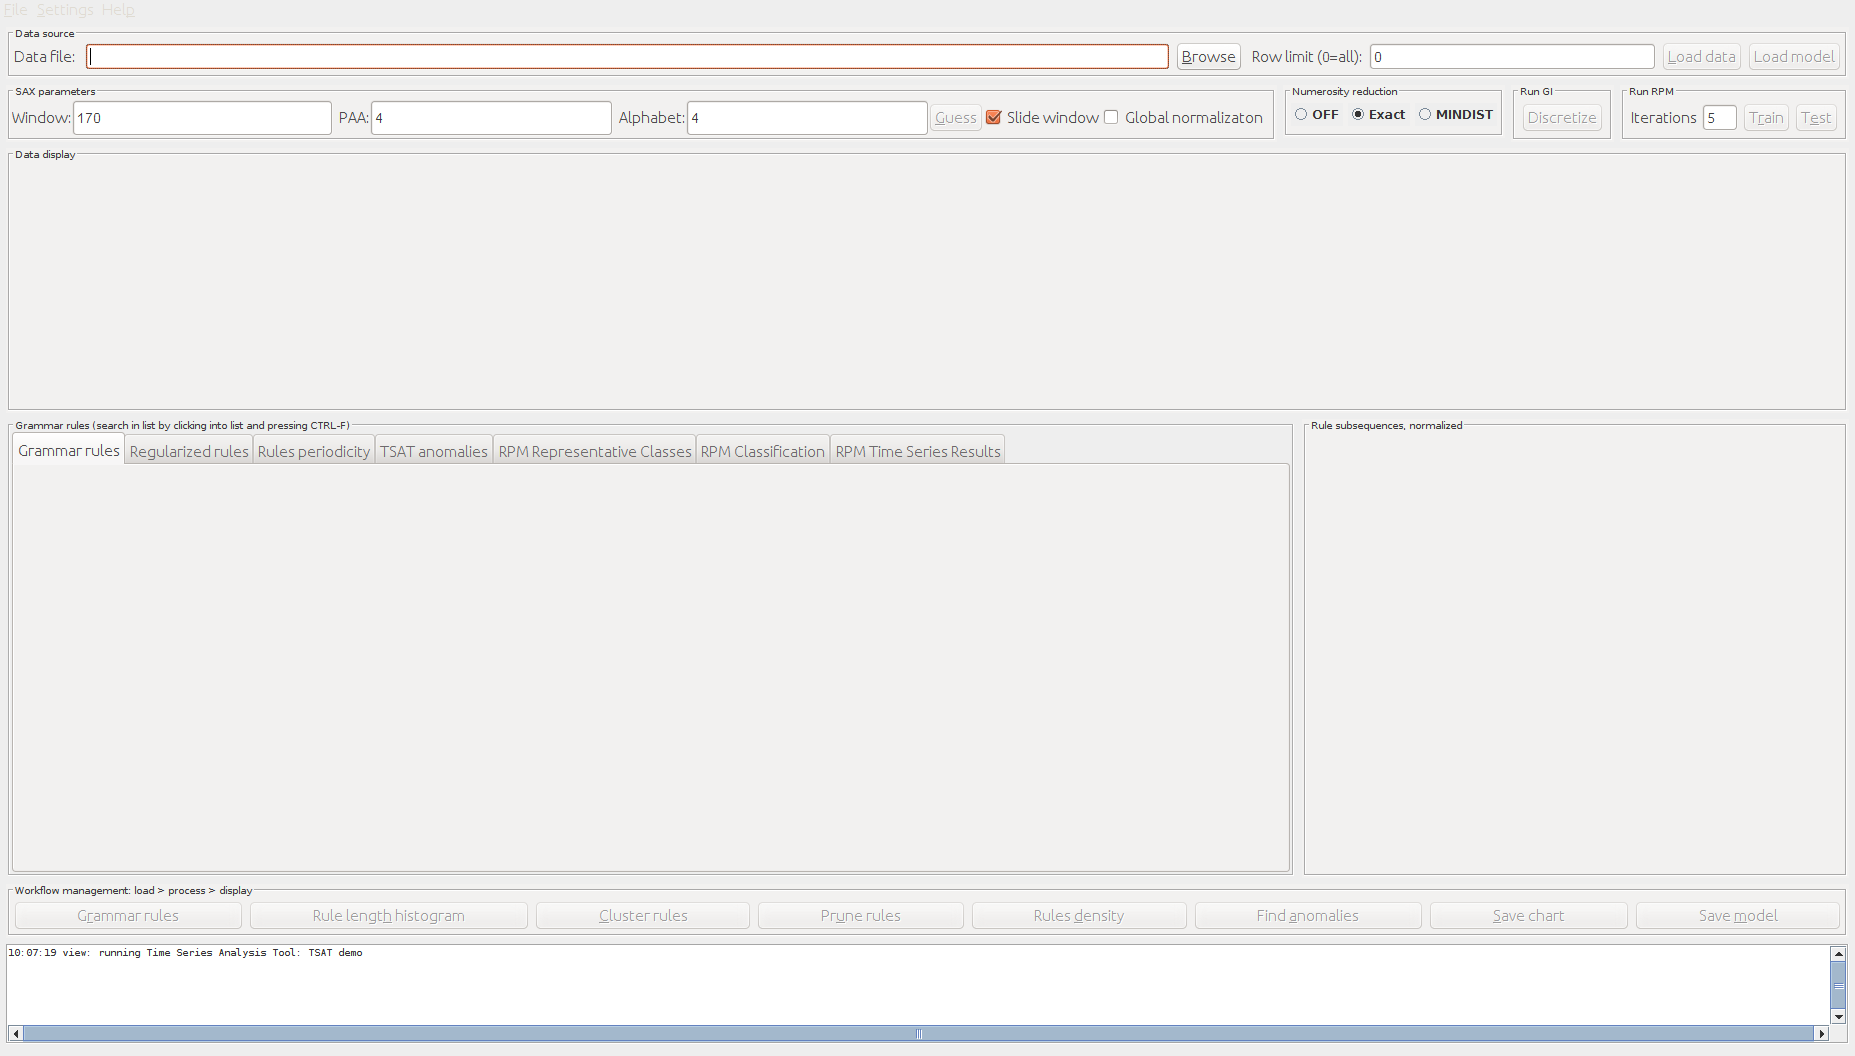
\includegraphics[width=\textwidth]{pictures/TSAT-interface}
	\caption{Initial state of the {\TSAT} Graphical User Interface (GUI).}
	\label{fig:tsat-interface}
\end{figure}

There are eleven regions in the main GUI used to set parameters, load files, and analyze results.  The nine main regions in the GUI have a rectangular outline around them with a label.  They include: ``Data Source'', ``SAX Parameters'', ``Numerosity reduction'', ``Run GI'', ``Run RPM'', ``Data display'', ``Grammar rules'', ``Rule Subsequences, normalized'', and ``Workflow management.''  The other two regions are the top menu bar (with ``File'', ``Settings'', and ``Help'') and the text area at the bottom of the GUI.  Presently, the items under ``Help'' do not have any meaningful functionality.  The text area at the bottom of the GUI is used to log useful information about the state of GUI.  That text area may also be referred to as the logging area.

\subsection{Tools Introduction}
{\TSAT} provides implementations of a number of algorithms used to analyze time series including Representative Pattern Mining (RPM) to perform time series classification, Motif Discovery to find repeating patterns, and Discord Discovery to detect anomalies.


\subsubsection{Motif Discovery}
A motif is a reoccurring pattern within a time series (an example motif is shown in Figure~\ref{fig:tsat-example-motif}) and both anomaly detection and representative pattern mining build from this concept.  In order to identify motifs within a time series {\TSAT} first converts the time series into a string (a sequence of words) and then performs context free grammar induction (GI).  Specifically {\TSAT} executes two main algorithms SAX (Symbolic Aggregate Approximation) with numerosity reduction and a user chosen GI algorithm either Sequitur or Re-Pair~\cite{senin-gv2,nevill1997identifying,larsson2000off}.  The motifs are then defined as the subsequences in the time series defined by the grammar rules.  {\TSAT} allows the user to explore the motifs by sorting by how frequently the rule is used in the root rule (labeled R0 in {\TSAT}).

\paragraph{SAX}SAX converts the time series into a string, or a sequence of characters.  It does this by using a fixed size sliding window over the time series and performing Piecewise Aggregate Approximation (PAA) on each window and converting those values into words.  This is called subsequence discretization~\cite{lonardi2002finding}.

First SAX splits the time series up into smaller time series by only looking at a fixed size window, or subsequence extraction as seen in Figure~\ref{fig:tsat-slidingwindow}.  So, if the time series is of length 1000 and the window length is 100 then each time series that SAX looks at is of length 100.  SAX uses a sliding window with a step size of one.  This means that the first time series given the same example spans from timestep 1 to 100 and the second time series is 2 to 101 and so there will be 999 different time series of length 100.  The formula is \(n - w + 1\) where \(n\) is the length of the time series and \(w\) is the length of the sliding window (the \textbf{window length}).

\begin{figure}[H]
	\centering
	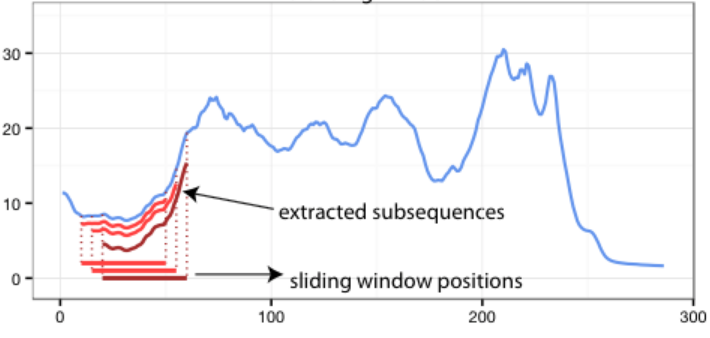
\includegraphics[width=0.7\textwidth]{pictures/TSAT-slidingwindow}
	\caption{Subsequence extraction from a sliding window.  Adopted from:\\ \url{http://grammarviz2.github.io/grammarviz2_site/morea/assets/sax-error.png}}
	\label{fig:tsat-slidingwindow}
\end{figure}


Then for each sliding window time series, PAA produces a word by first performing z-normalization on the values.  This means converting the time series values to values with a mean and standard deviate of approximately 0 and 1 respectively.  However, so as to not amplify the ``under-threshold-noise'' there is a \textbf{z-normalization threshold} value so that if the input time series' standard deviation is less than this value the z-normalization will not be applied. Then the algorithm splits the window up into \(m\) equal sized segments called the \textbf{PAA size} and for each of the segments it computes the mean value.  

SAX maps each mean value to a letter in the alphabet and produces a word (a sequence of letters/characters).  The number of characters, \(a\), available in the alphabet is chosen by the user (the \textbf{alphabet size}).  Since the values of z-normalized time series follow the Normal distribution~\cite{lin2003symbolic}, the breakpoints for each character can be determined by making \(a\) equal-sized areas under the Normal curve using lookup tables (illustrated along the y-axis in Figure~\ref{fig:tsat-sax}). Then for each of the windows we have created a word.  Figure~\ref{fig:tsat-sax} shows the process of converting a time series (without any sliding window) into a SAX word.  It should be pointed out that the ``observation that normalized subsequences have highly Gaussian distribution, is not critical to correctness of any of the algorithms that use SAX, including the ones in this work. A pathological dataset that violates this assumption will only affect the efficiency of the algorithms''~\cite{keogh2004hot}.

\begin{figure}[H]
	\centering
	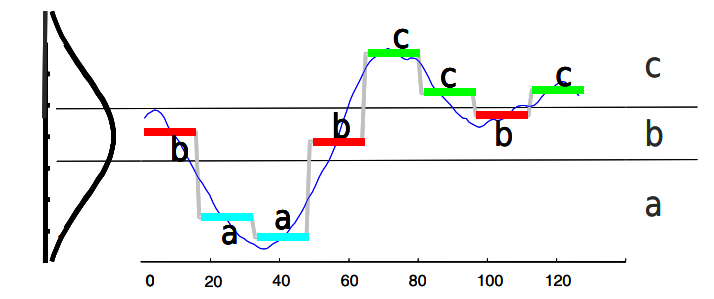
\includegraphics[width=.7\textwidth]{pictures/TSAT-SAX}
	\caption{``A time series is discretized by first obtaining a PAA approximation and then using predetermined breakpoints to map the PAA coefficients into SAX symbols. In the example above, with n = 128, w = 8 and a = 3, the time series is mapped to the word baabccbc.''  Both the figure and the included caption are from~\cite{lin2007experiencing}.}
	\label{fig:tsat-sax}
\end{figure}


\paragraph{Numerosity Reduction}The list of words produced using this procedure is also compressed using numerosity reduction.  Numerosity reduction reduces the size of this list of words by skipping duplicate words.  Additionally, ``numerosity reduction makes motif discovery more robust, as we are matching patterns based on their shapes, even if they do not have the exact same lengths''~\cite{li2012visualizing}.  For example, a time series \(S_{1}\) 

\[
S_{1}= aac_{1}\, aac_{2}\, abc_{3}\, abb_{4}\, acd_{5}\, aac_{6}\, aac_{7}\, aac_{8}\, abc_{9}\, \dots
\]
is converted to the much smaller string using numerosity reduction:
\[S2 = \textit{aac}_{1}~ \textit{abc}_{3}~ \textit{abb}_{4}~ \textit{acd}_{5}~ \textit{aac}_{6}~ \textit{abc}_{9}\]
where the subscripts are the window numbers.

\paragraph{Grammar Induction GI}Then grammar induction is used to produce grammar rules, the motifs, from the SAX string. Both Sequitur and Re-Pair are context free grammar induction algorithms that are included in {\TSAT}.  {\TSAT} uses Sequitur as its default.  However, there are a number of differences according to~\cite{readmeGI}:
\begin{itemize}
	\item Sequitur implementation is slower than Re-Pair
	\item Sequitur tends to produce more rules, but Sequitur rules are less frequent than Re-Pair rules
	\item Sequitur rule-corresponding subsequences vary in length more
	\item Sequitur rules usually cover more points than Re-Pair
	\item Sequitur rule coverage depth is lower than that of Re-Pair
\end{itemize}

A simple example (not a time series) of a context free grammar is to take the following string ``a rose is a rose is a rose'' this can be converted to the following grammar rules:

\begin{center}
	S \(\rightarrow\) BBA\\
	A \(\rightarrow\) B is\\
	B \(\rightarrow\) a rose\\
\end{center}
Where S is the root rule, meaning that no rule uses this rule and A and B are grammar rules that are used in S. Also, note that the grammar forms a hierarchy and therefore will not contain cycles.  As the above example illustrates the lengths of the motifs can be of varying lengths as the rule may contain other rules (note that in an actual time series each word would be the same length).
\begin{figure}[H]
	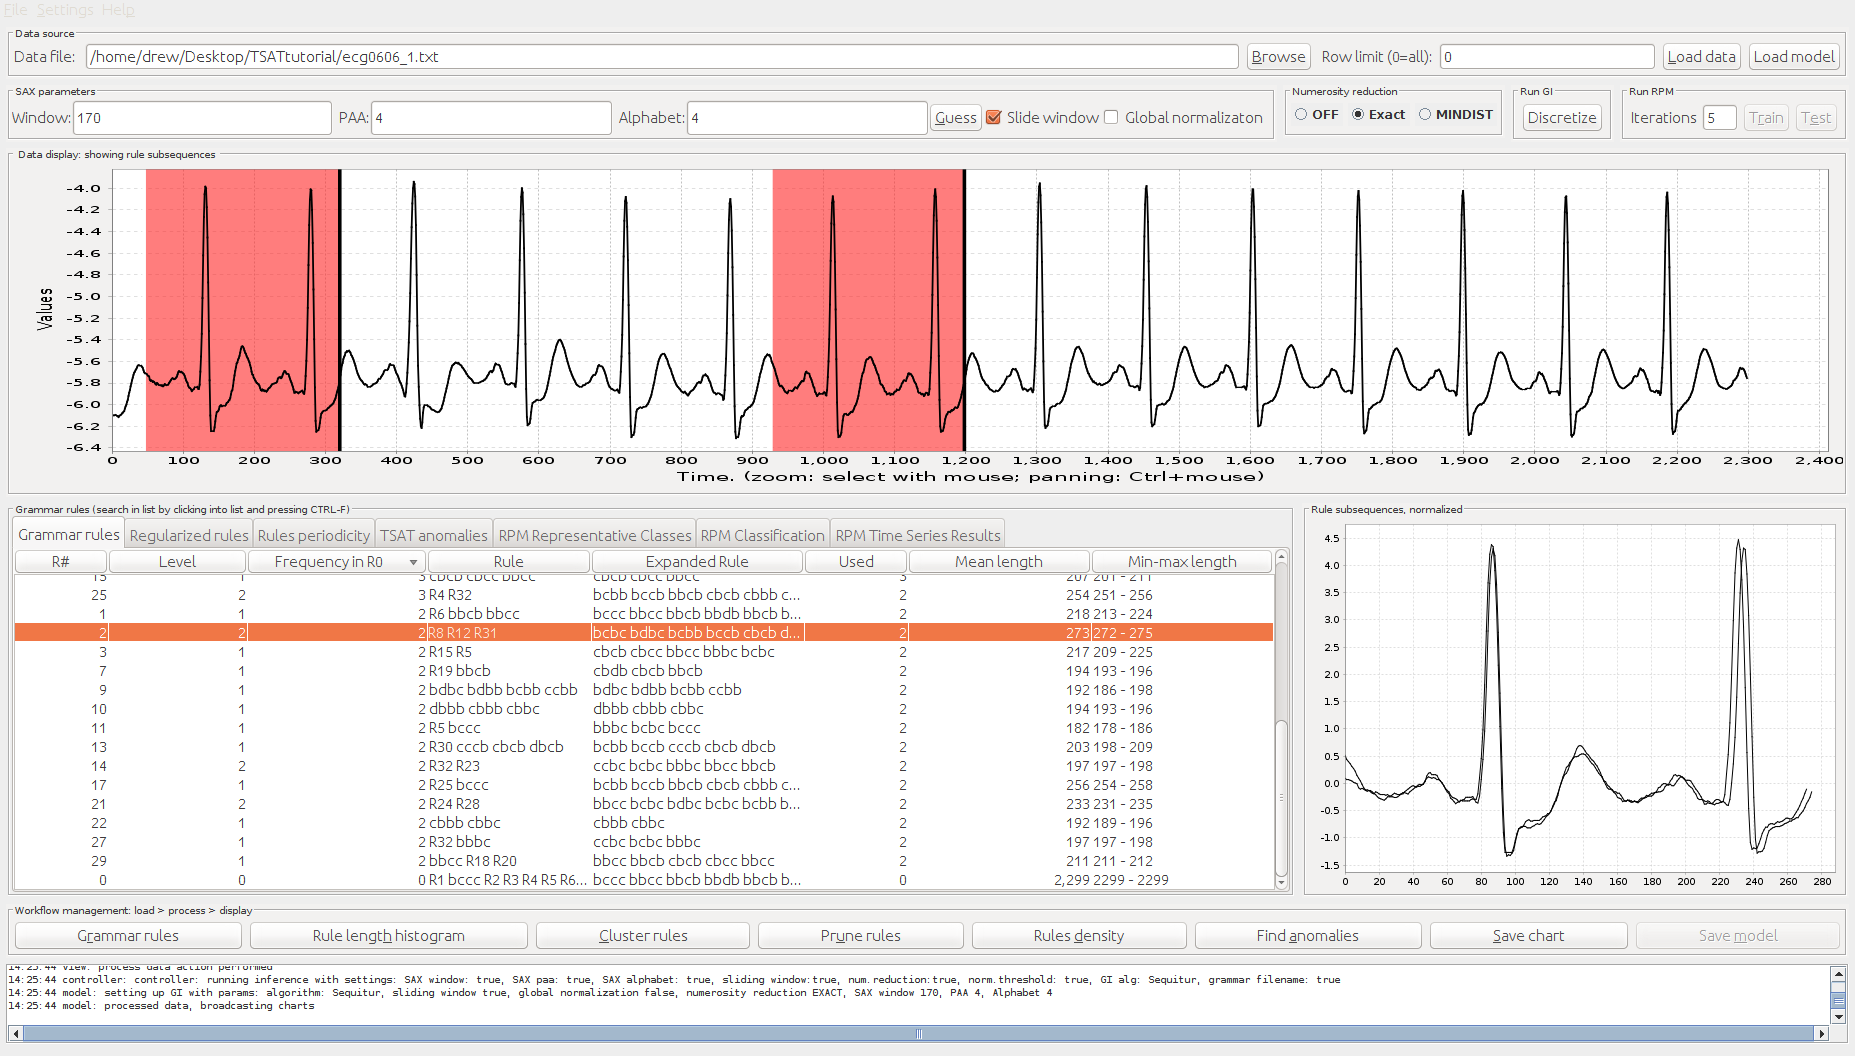
\includegraphics[width=\textwidth]{pictures/TSAT-example-motif}
	\caption{Example motif found using {\TSAT} with the subsequences highlighted in the Data Display and shown in the Rules Subsequences areas.}
	\label{fig:tsat-example-motif}
\end{figure}
\paragraph{Setting the Parameters}One example motif found by {\TSAT} in ECG data is shown in Figure~\ref{fig:tsat-example-motif}.  There are only three parameters, alphabet size, PAA length, and window size.  Past studies have empirically shown that an alphabet size of 3 or 4 will work in most settings and that the PAA length depends on the data.  The PAA length (also known as word size) tends to be a smaller value for smooth and slow changing time series and a larger value for more complex time series~\cite{keogh2004hot}. ``Note however, that grammar induction step effectively mitigates improper sliding window selection''~\cite{motifSite}.


\subsubsection{Anomaly Detection}

%Anomalies are discords the subsequences whose distance to their nearest non-self match is the largest.

%anomalous subsequences correspond to rare grammar rules, we call the algorithm RRA (Rare Rule Anomaly)

%A subsequence is a non-self match with another subsequence if there subsequences do not overlap

{\TSAT} also implements two anomaly detection algorithms taking an exact approach and an approximate approach~\cite{senin2015time}.  Specifically the \textbf{Rare Rule Anomaly} (RRA) algorithm and the \textbf{rule density curve} algorithm.  Each method uses the grammar rules generated by Sequitur or Re-Pair to extract the corresponding subsequences in the time series.  However, each method uses these subsequences in a different way.

RRA defines anomalous subsequences as \textit{discords} or the subsequences whose euclidean distance (normalized by the subsequence length) to their nearest non-self match is the largest.  A subsequence is a non-self match with another subsequence if their subsequences do not overlap. 

The approximate anomaly detection method is implemented using the rule density curve.  The value at each point in the rule density curve is the number of grammar rules that span or ``cover'' the corresponding point in the time series.  Therefore, ``rule density curve intervals that contain minimal values correspond to time series anomalies''~\cite{senin2015time}.  

Both the exact and approximate methods can find variable length anomalies.  However, ``if the time series under analysis has low regularity (an issue that impacts the grammar’s hierarchy) or the discretization parameters are far from optimal and regularities are not conveyed into the discretized space, the rule density based anomaly discovery technique may fail to output true anomalies''~\cite{senin2015time}.  Therefore, using the exact approach is preferable.
\paragraph{Setting the Parameters} The best advice is from~\cite{senin2015time}:

\begin{quote}
	Specifically, we found that the rule density curve facilitates the discovery of patterns that are much shorter than the window size, whereas the RRA algorithm naturally enables the discovery of longer patterns. Second, we observed that when the selection of discretization parameters is driven by the context, such as using the length of a heartbeat in ECG data, a weekly duration in power consumption data, or an observed phenomenon cycle length in telemetry, sensible results are usually produced.
\end{quote}


\subsubsection{Representative Pattern Mining - RPM}
\label{RPMOverview}



\subsection{Overview}

\section{Time Series Classification using RPM}
TSAT implements Representative Pattern Mining or RPM  (see Section~\ref{RPMOverview} for more details) to perform time series classification.  In order to perform time series classification you will need a training and a test dataset containing time series data.

The standard method to train a supervised learning classifier is to take the labeled dataset and split it into two datasets, training and testing data.  One common way to split the data is to have 80\% training and 20\% testing.  

\paragraph{Training Data}
Training data is the primary data and will be used to create a model that can identify similar patterns in new, unlabeled, data. This data must have a label for each time series so that RPM can learn what the labels can look like. This is where the bulk of the data should be set aside for as RPM will need many samples to find representative patterns.

\paragraph{Testing Data}
Testing data is a small subset of the data usually from the same source as the training data, but not found in the training data. This set of data will be used to test the model that RPM made for accuracy or to predict labels for unlabeled test data.

Splitting data into a training and a test set is beyond the scope of this manual and is not done by TSAT. The goal of this section is to first detail the proper file formats for training and testing data in Section~\ref{RPMFile}. Then the proper procedures to train (Section~\ref{RPMTrain}), test (Section~\ref{RPMTest}), and review the results (Section~\ref{RPMResults}) are presented step by step. 

\subsection{File formats}
\label{RPMFile}
File formatting is very important in TSAT and especially when using RPM.  If the file is not in the correct format TSAT will not be able to read the file and may produce unexpected results or error messages.  The data may be formatted by column, row, or following the ARFF file format. Additionally, the labels for the time series may be any string excluding white space and ``?'' as this is reserved for unknown values in test data.

\begin{figure}[h]
	\caption{Examples of RPM Data}
	\label{fig:rpm-data-exs}
	\begin{subfigure}[b]{0.5\textwidth}
		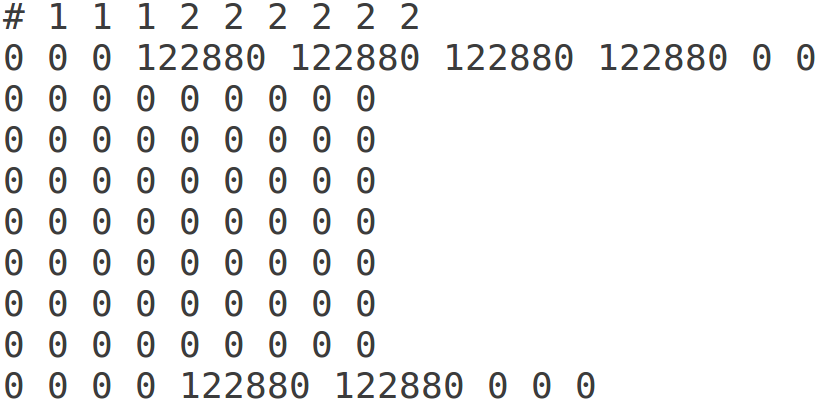
\includegraphics[width=\textwidth]{rpm_data_example_1}
		\caption{Example 1}
		\label{fig:rpm-data-ex-1}
	\end{subfigure}
	~
	\begin{subfigure}[b]{0.5\textwidth}
		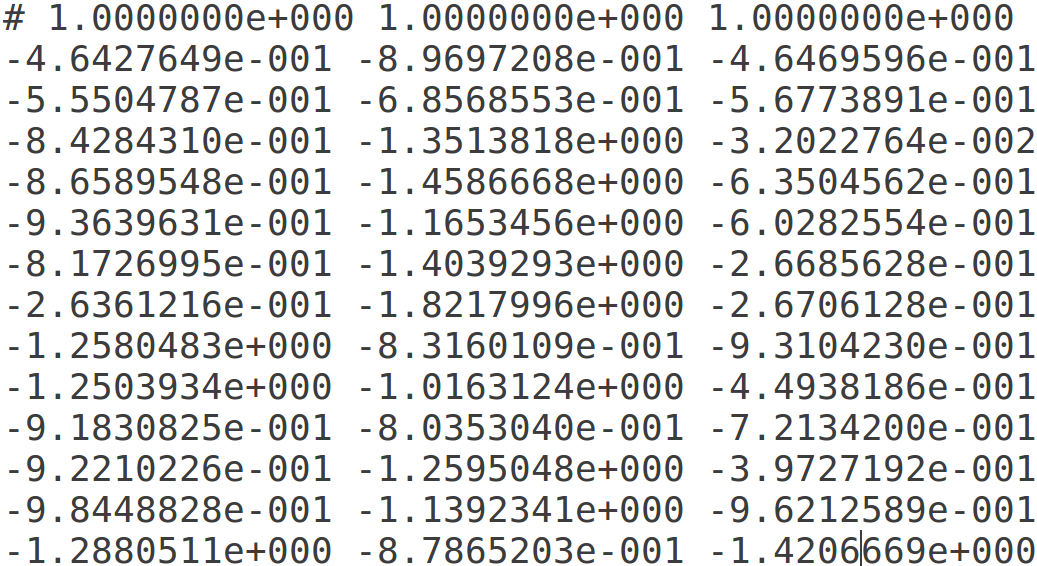
\includegraphics[width=\textwidth]{rpm_data_example_2}
		\caption{Example 2}
		\label{fig:rpm-data-ex-2}
	\end{subfigure}
\end{figure}

\paragraph{Column Formatted Data}
The data files are simple text files that store the time series data with one entry per column, with a space delimiter, with each row representing a time step in the time series data. With RPM compatible data the first row in the file starts with a ``\#'' with rest of the row containing the label for each time series rather then the time series values. If the file is missing this row RPM will not be enabled in TSAT. Examples of column formatted RPM compatible data can be seen in figure~\ref{fig:rpm-data-exs}.  Another thing to keep in mind is that in this format the time series must all be the same length. 

\paragraph{Row Formatted Data}
Another acceptable format is the row format.  This format is especially useful  when the time series are not all the same length as each row or time series may have its own length.  In this format the first line of the file is a ``\#'' followed by a new line.  Starting on the second line, each line starts with the label followed by the corresponding time series (each value separated by a space).  There should be no empty lines.  For example,\\
%\newpage
\begin{allintypewriter}
	\noindent\#\\
	1 -5.3 -23 5 ...\\
	1 23 1 5 3 1 ...\\
	two 23 3 4 200 ...\\
	two 42 3 4 102 ...\\
	...
\end{allintypewriter}
In this example the labels are ``1'' and ``two'' and the time series follow after the labels.

\paragraph{ARFF Formatted data}

A standard format for many public time series datasets is the ARFF file format.  For example, \url{http://timeseriesclassification.com/dataset.php} has a number of time series in ARFF format that can be used in TSAT.  ARFF files are more complicated than both the column and row formats, but is more widely used outside TSAT.  Here is an abbreviated example ARFF file:
\begin{samepage}
\begin{allintypewriter}
	\noindent @relation Adiac\\ \\
	@attribute att0 numeric\\
	@attribute att1 numeric\\
	...\\
	@attribute target {1,2,...}\\ \\
	@data\\
	1.3749,1.2894,1.2043,1.1194,1.0347, ... 1\\
	1.7257,1.7001,1.6611,1.6089,1.5319, ... 2\\
	...
\end{allintypewriter}
\end{samepage}
The ARFF file begins with the name of the dataset Adiac by using the ARFF formatting by putting it after the \texttt{@relation} element. After the name of the dataset each timestep is listed as an attribute \texttt{@attribute <timestepName> numeric} where you can choose what to name each timestep. After listing the timesteps as attributes the labels are listed as the target attribute \texttt{@attribute target \{1, 2, ...\}} where these are the labels for the time series. Finally, the time series data is in comma separated value (CSV) format following the \texttt{@data} line.  Each value in a time series is separated by a comma on a single line and the last value on the line is the label for the time series.

\paragraph{Unknown Test Data}
In column, row, or ARFF format when predicting unlabeled test data, the test data must be labeled as ``?'' (note that there must only be test data that is labeled with a ``?'').  For example, a row formatted test dataset might be:

\begin{allintypewriter}
	\noindent\#\\
	? -5.3 -23 5 ...\\
	? 23 1 5 3 1 ...\\
	? 23 3 4 200 ...\\
	...
\end{allintypewriter}

As can be seen the label is ``?'' and the time series follows after the label.  When training there must always be more than one example from each class label and there must be more than one label.

\subsection{Training}
\label{RPMTrain}

Once you have the data in the proper format and TSAT open training RPM can begin.

\paragraph{Step 1}
First click on the ``Browse'' button under the ``Data Sources'' section of the window, as seen in figure \ref{fig:TSAT-training-step-1}. 

\begin{figure}[h]
	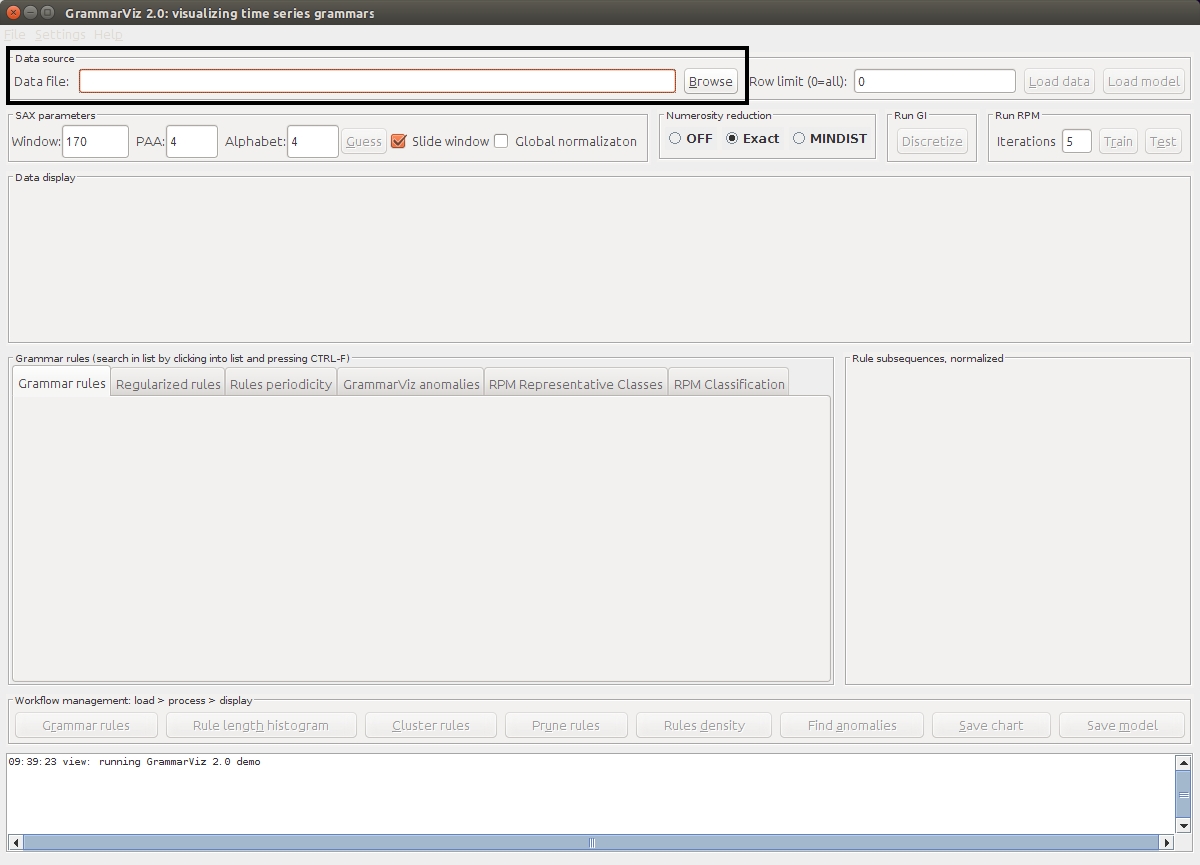
\includegraphics[width=\textwidth]{TSAT-training-step-1}
	\caption{Open TSAT}
	\label{fig:TSAT-training-step-1}
\end{figure}
\newpage
\paragraph{Step 2}
This should bring up the file browser prompt in figure \ref{fig:TSAT-training-step-2}. Using this prompt select the file containing the training set in the RPM compatible format, figure \ref{fig:TSAT-training-step-3}.

\begin{figure}[H]
	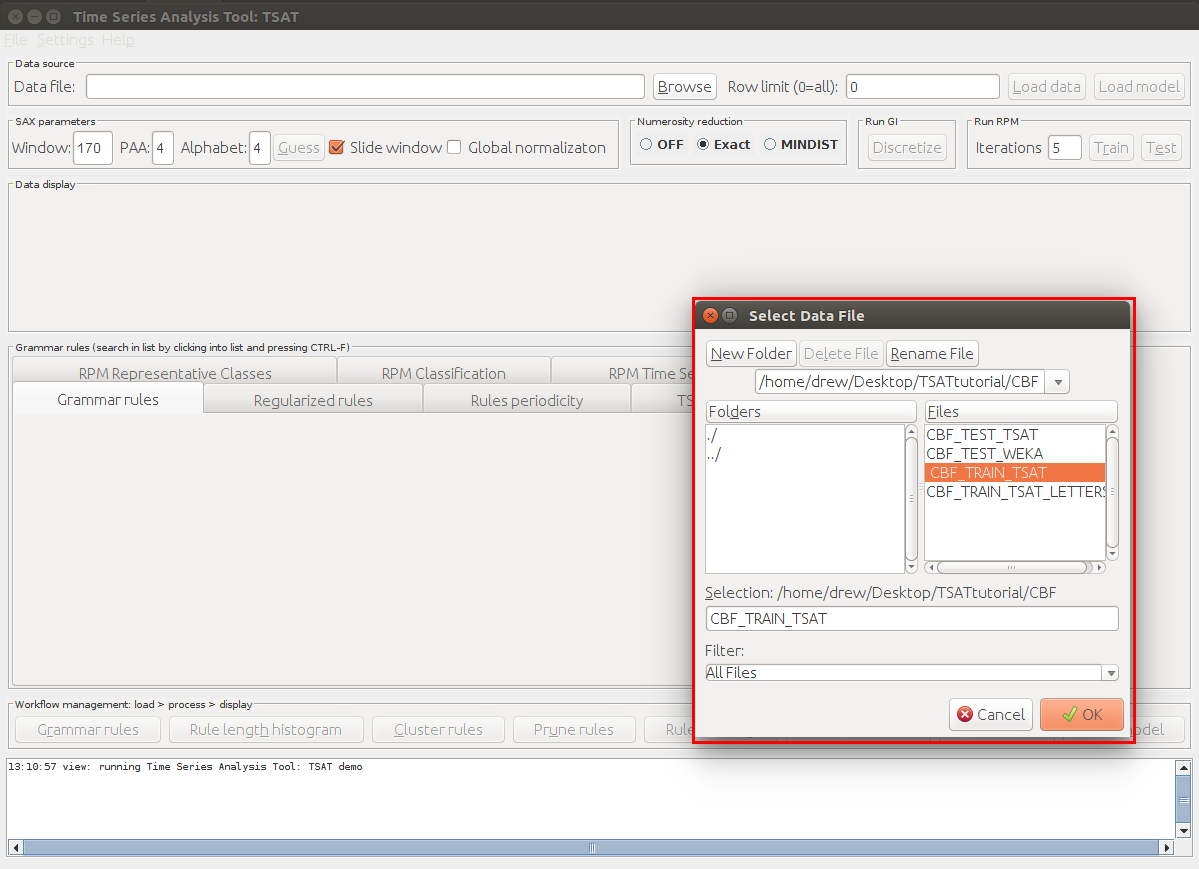
\includegraphics[width=\textwidth]{TSAT-training-step-2}
	\caption{Open the file browser prompt}
	\label{fig:TSAT-training-step-2}
\end{figure}
\begin{figure}[H]
	\center
	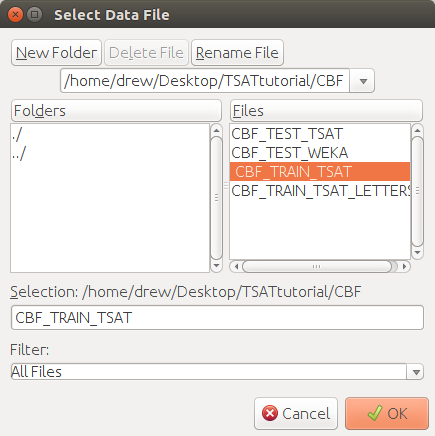
\includegraphics[width=.4\textwidth]{TSAT-training-step-3}
	\caption{Browser prompt}
	\label{fig:TSAT-training-step-3}
\end{figure}

\newpage
\paragraph{Step 3}
After selecting the file press the button labeled ``Load Data'' and  TSAT will load the data and the graphs will be populated, and if the data is found to be RPM compatible data then the ``Train'' button should become available. The text field labeled ``Row Limit'' allows the user to limit the number of rows that are read in from file, for example if the file contains 100 rows the user could limit it to the first 50. 

\begin{figure}[H]
	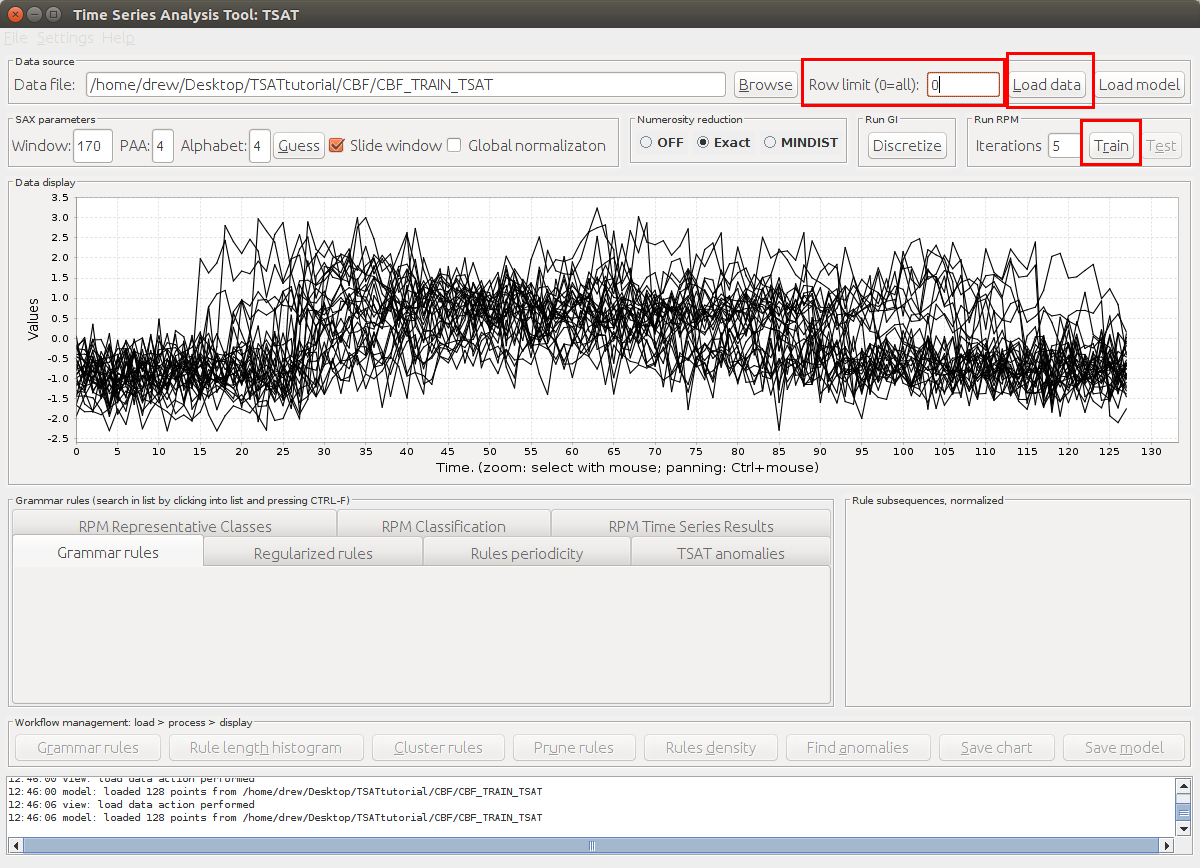
\includegraphics[width=\textwidth]{TSAT-training-step-4}
	\caption{Loaded data}
	\label{fig:TSAT-training-step-4}
\end{figure}

\newpage
Hitting this button will begin the training phase of RPM, this can take some time depending on the data and the number of iterations RPM will run. The text field labeled ``Iterations'' sets the maximum number of iterations RPM will go, this prevents RPM from running for to long trying to refine the model. Once the training is complete the tab ``RPM Representative Classes'' will become populated with patterns RPM thinks be represent the labels given. The fields ``Window'', ``PAA'', and ``Alphabet'' will also be populated with the values RPM believes are the best fit for the data to aid in further analysis. 

\begin{figure}[H]
	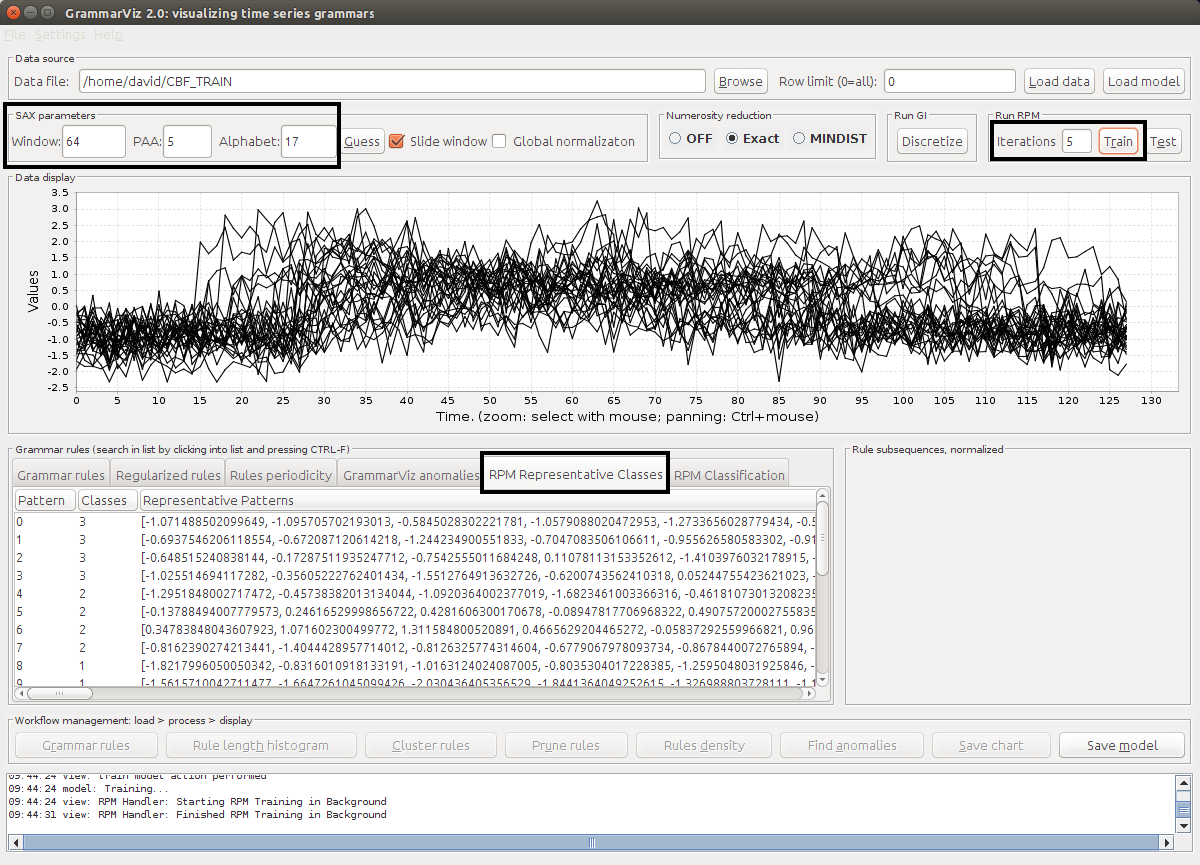
\includegraphics[width=\textwidth]{TSAT-training-step-5}
	\caption{Representative Classes after Training}
	\label{fig:TSAT-training-step-5}
\end{figure}

\newpage
Selecting the patterns will display their graph on the right hand side of the window, multiple patterns can be selected.

\begin{figure}[H]
	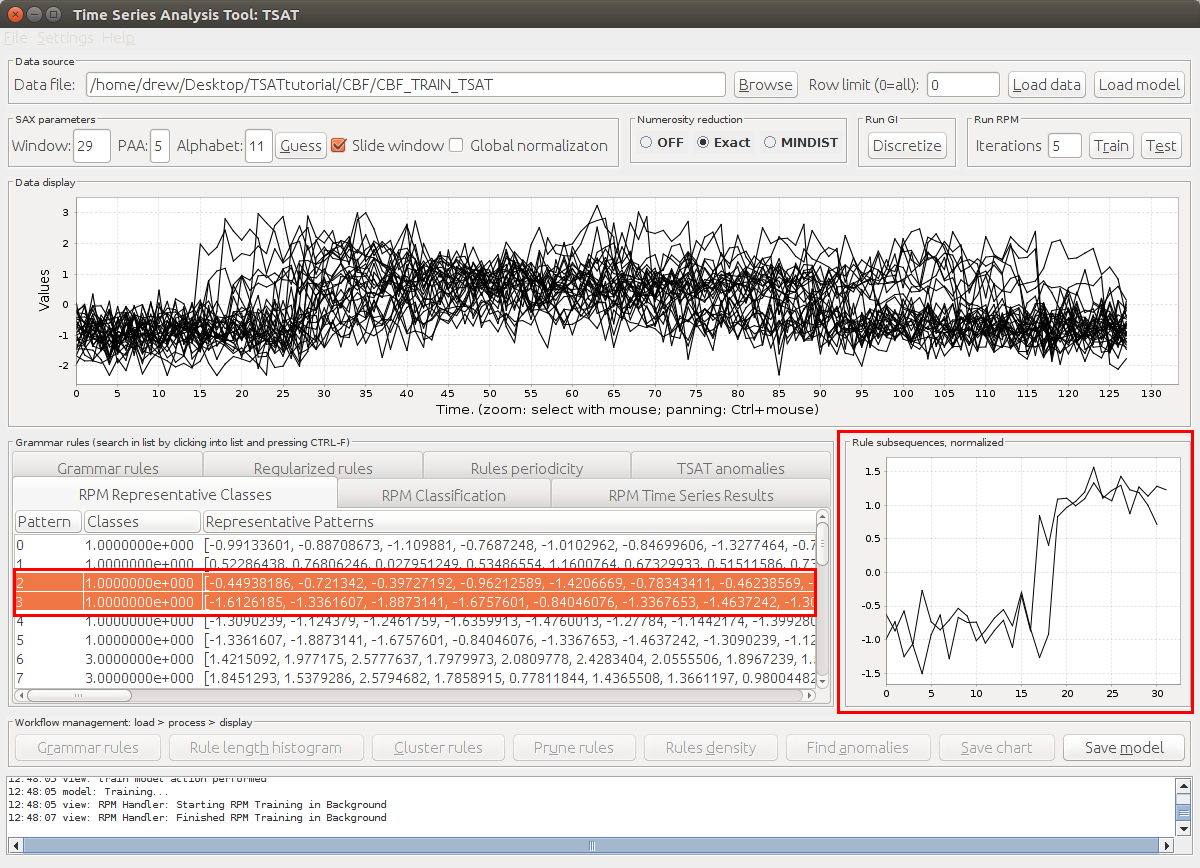
\includegraphics[width=\textwidth]{TSAT-training-step-6}
	\caption{Representative pattern preview}
	\label{fig:TSAT-training-step-6}
\end{figure}


\subsection{Testing}
\label{RPMTest}
Once the model has be trained it should be tested for accuracy, this will use a smaller dataset in the RPM compatible format to measure how well the model does. 

\paragraph{Step 1}
Click the ``Test'' button and a file browser prompt will appear, depending on how large the dataset is this may take a moment. 

\begin{figure}[H]
	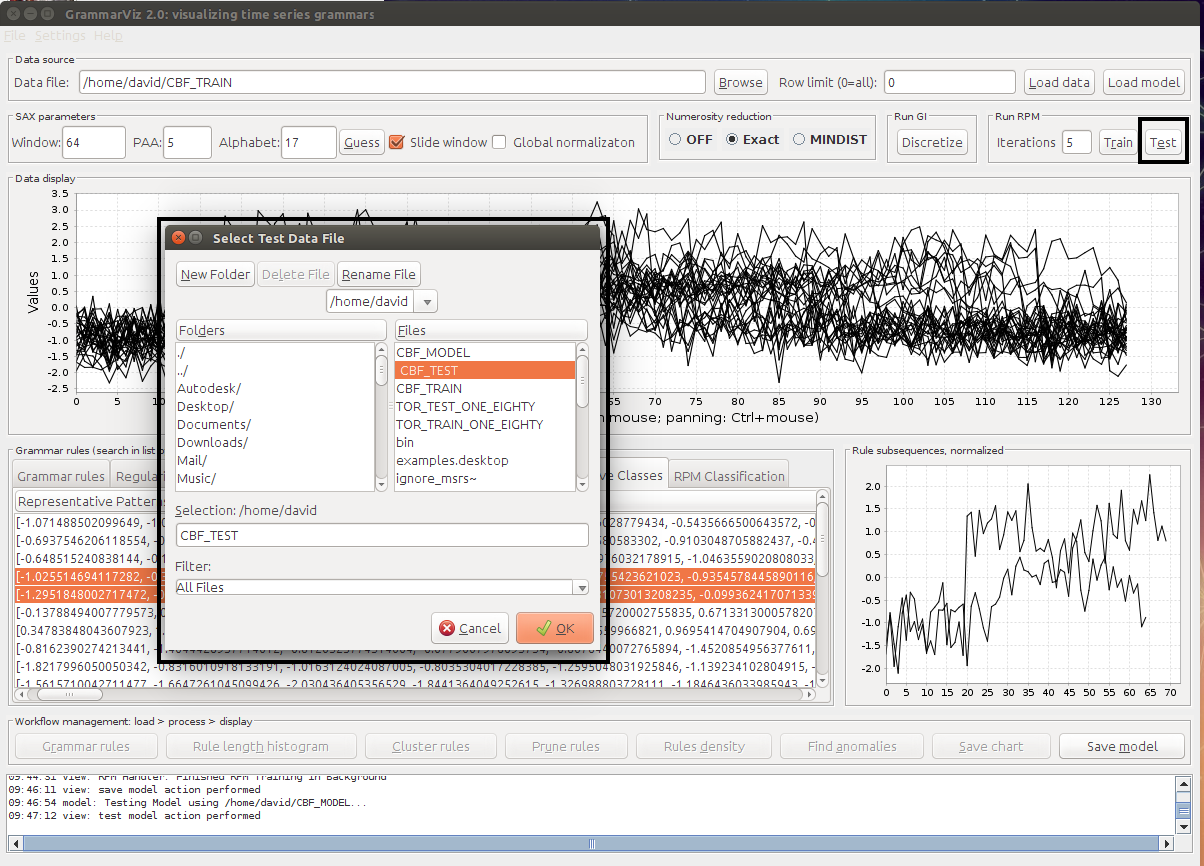
\includegraphics[width=\textwidth]{TSAT-testing-step-1}
	\caption{Testing the RPM model}
	\label{fig:TSAT-testing-step-1}
\end{figure}

\newpage
Once the testing is complete the tab labeled ``RPM Classification'' will be populated. This provides statistics on the effectiveness of the model by reporting the number of samples that were incorrectly labeled by the model.

\begin{figure}[H]
	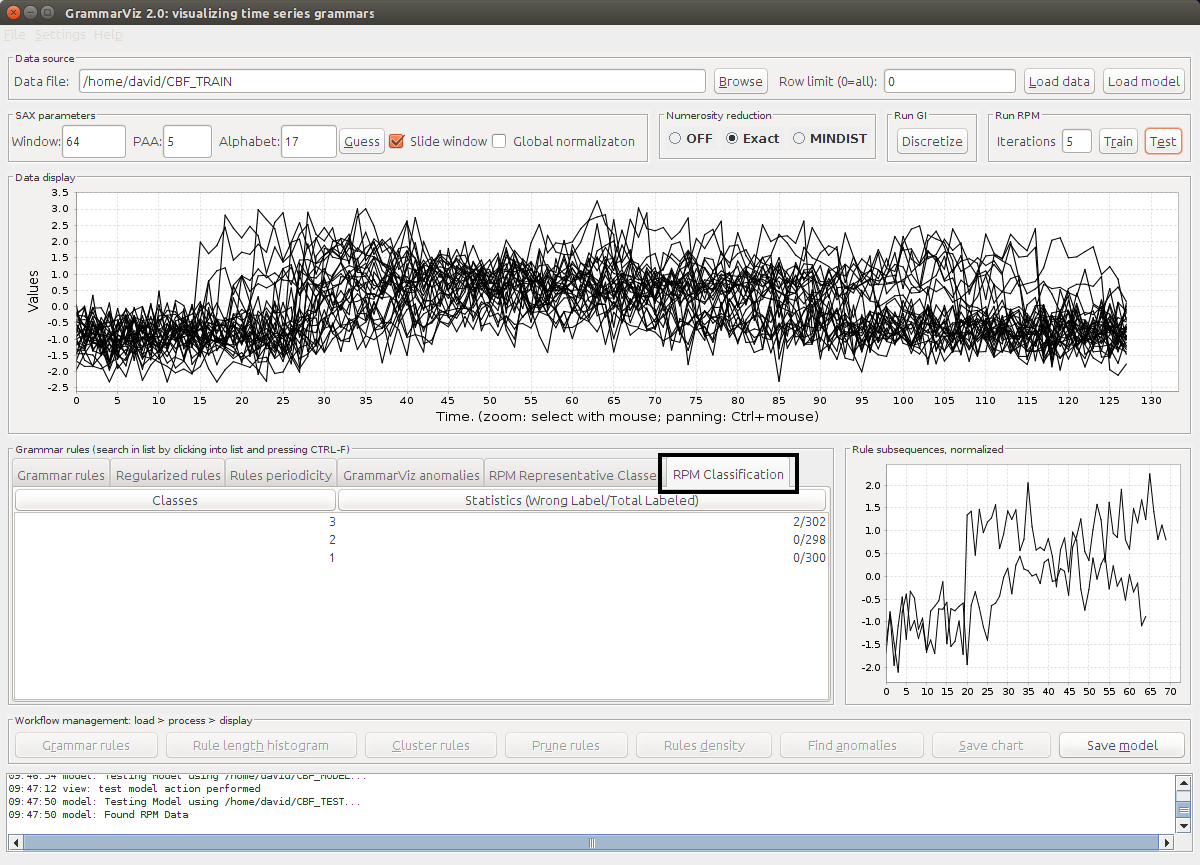
\includegraphics[width=\textwidth]{TSAT-testing-step-2}
	\caption{The results from the testing}
	\label{fig:TSAT-testing-step-2}
\end{figure}

\subsection{Testing Unlabeled Data}
Using the same method for loading the test data when the data is labeled we can see the results for unlabeled data.  Here the test data labels are all question marks so the results will consist of the probability that the test example is in each of the different training classes and the predicted label.  For example, in figure \ref{fig:TSAT-Results-Unknown-Test} the solid box has the label probability for each class and dashed box has the predicted class label.
\begin{figure}[H]
	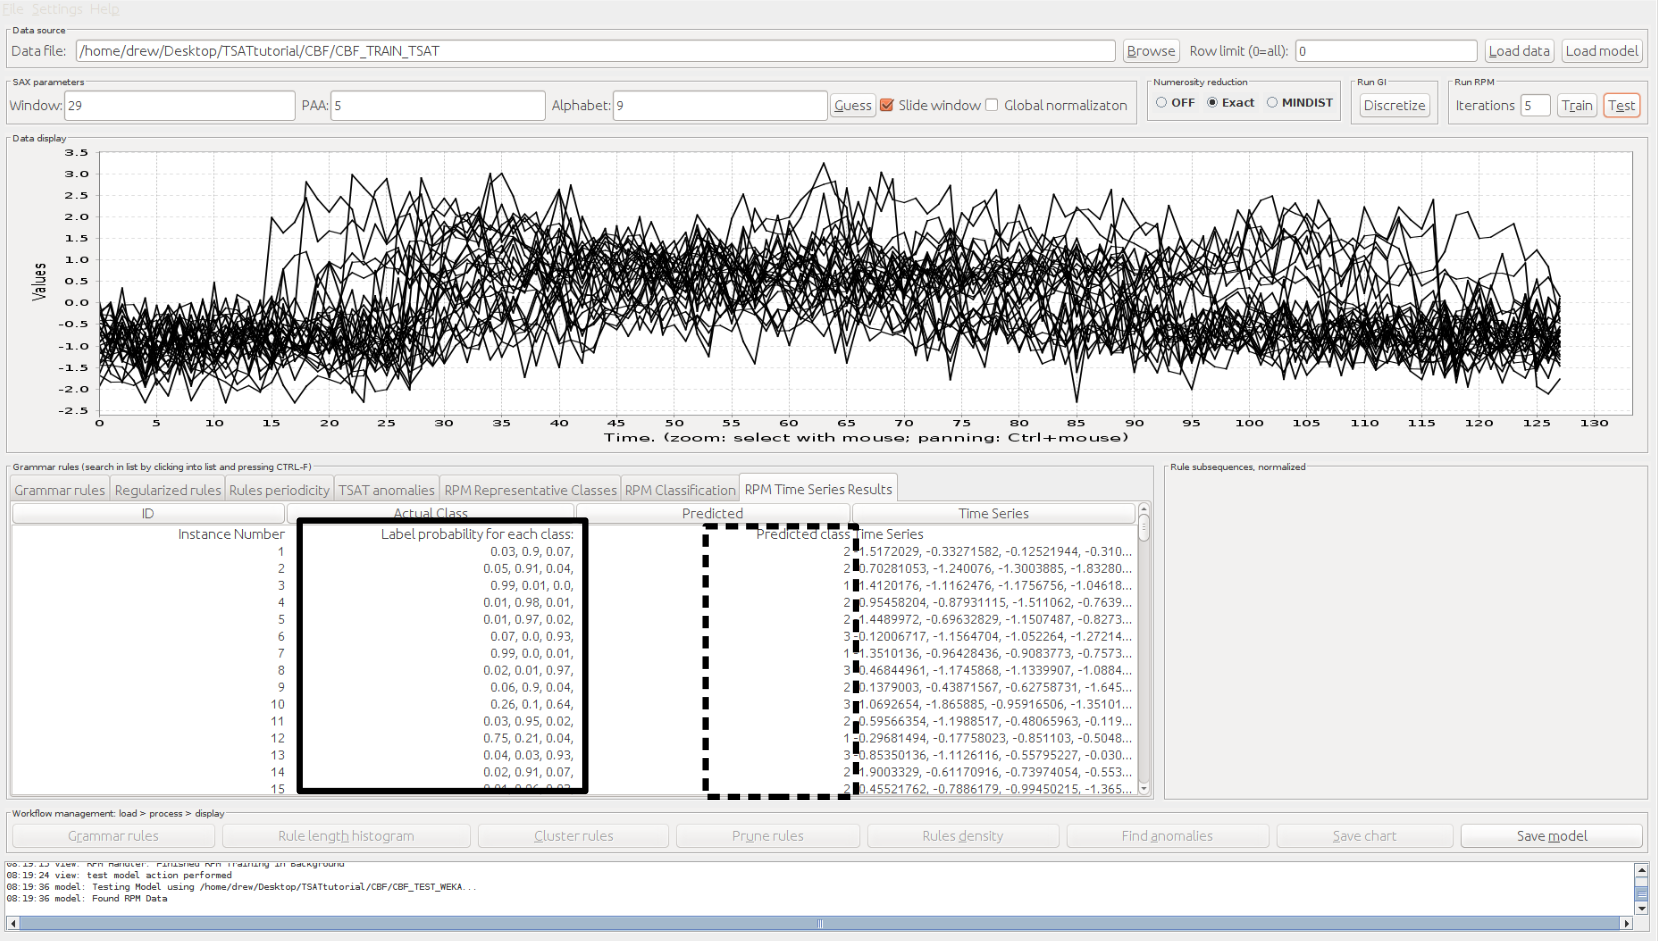
\includegraphics[width=\textwidth]{RPMTimeSeriesResultsUnknown}
	\caption{Solid box highlights the probability that the time series was in each of the different class labels and the dashed box highlights the predicted label.}
	\label{fig:TSAT-Results-Unknown-Test}
\end{figure}

\subsection{Saving a Trained RPM Model}
\label{RPMSaving}
Creating a model can take some time and there for being able to save the model for later uses is a useful feature. Saving the RPM model will generate a file that can be loaded in later for further testing. One thing to note is that the saved model does not contain the training data however the training data is still needed when doing testing there for a copy of the training data must be retained.

\paragraph{Step 1}
Once a model has been trained up clicking the save model button, as in figure \ref{fig:TSAT-save-model-step-1}, a file browser prompt will appear.

\begin{figure}[H]
	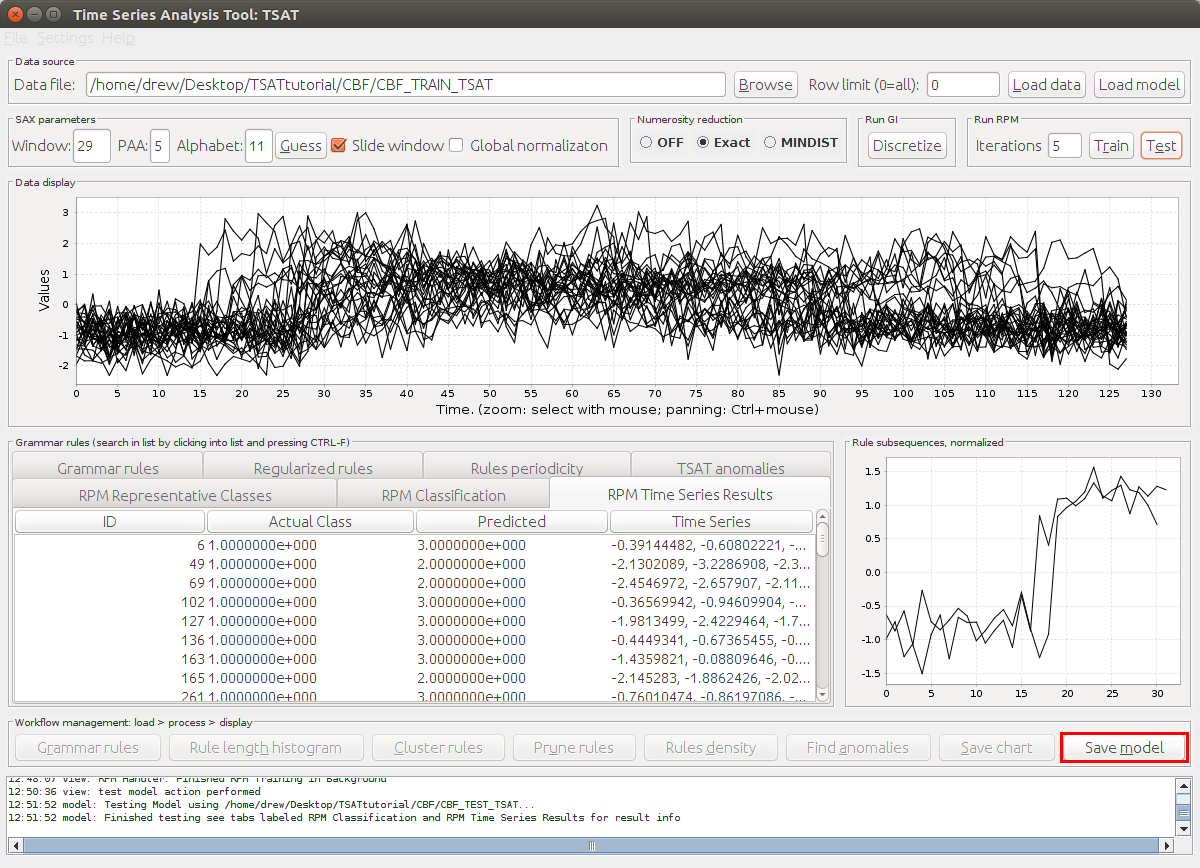
\includegraphics[width=\textwidth]{TSAT-save-model-step-1}
	\caption{Saving the RPM model}
	\label{fig:TSAT-save-model-step-1}
\end{figure}

\newpage
\paragraph{Step 2}
With the file browser prompt select a location to save the model and give it a name, then click the ``OK'' button to save the model.

\begin{figure}[H]
	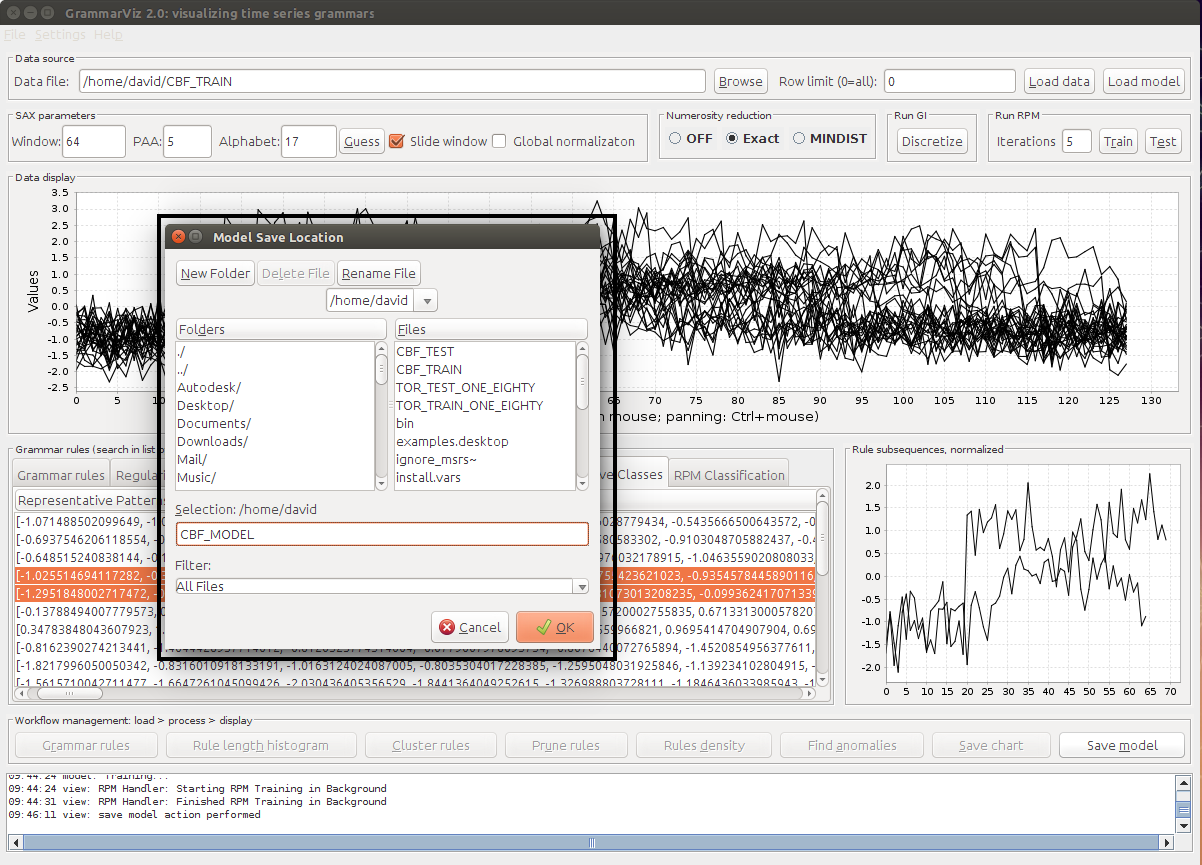
\includegraphics[width=\textwidth]{TSAT-save-model-step-2}
	\caption{Saving the RPM model to file}
	\label{fig:TSAT-save-model-step-2}
\end{figure}

\newpage
\subsection{Loading an RPM Model}
\label{RPMLoading}
When a model has already been saved, simply loading the will allow for further testing. When loading a model the software will look for the original training data from where it was when it was originally trained. If the data is not there then the software will ask for the location of the data.

\paragraph{Step 1}
First click on the ``Browse'' button under the ``Data Sources'' section of the window, as seen in figure \ref{fig:TSAT-load-model-step-1}. 

\begin{figure}[h]
	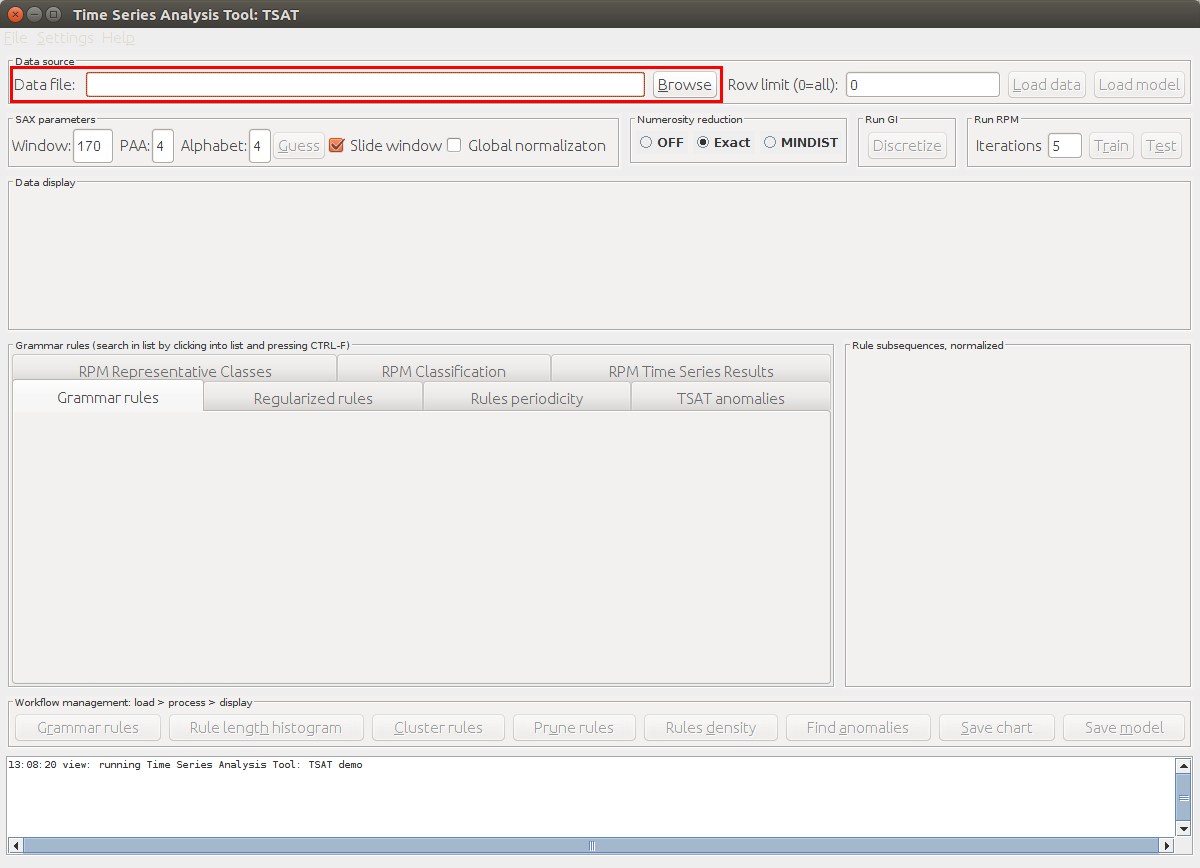
\includegraphics[width=\textwidth]{TSAT-load-model-step-1}
	\caption{Loading a model}
	\label{fig:TSAT-load-model-step-1}
\end{figure}

\newpage
\paragraph{Step 2}
This should being up the file browser prompt in figure \ref{fig:TSAT-load-model-step-2}. Using this prompt select the previously saved model.

\begin{figure}[H]
	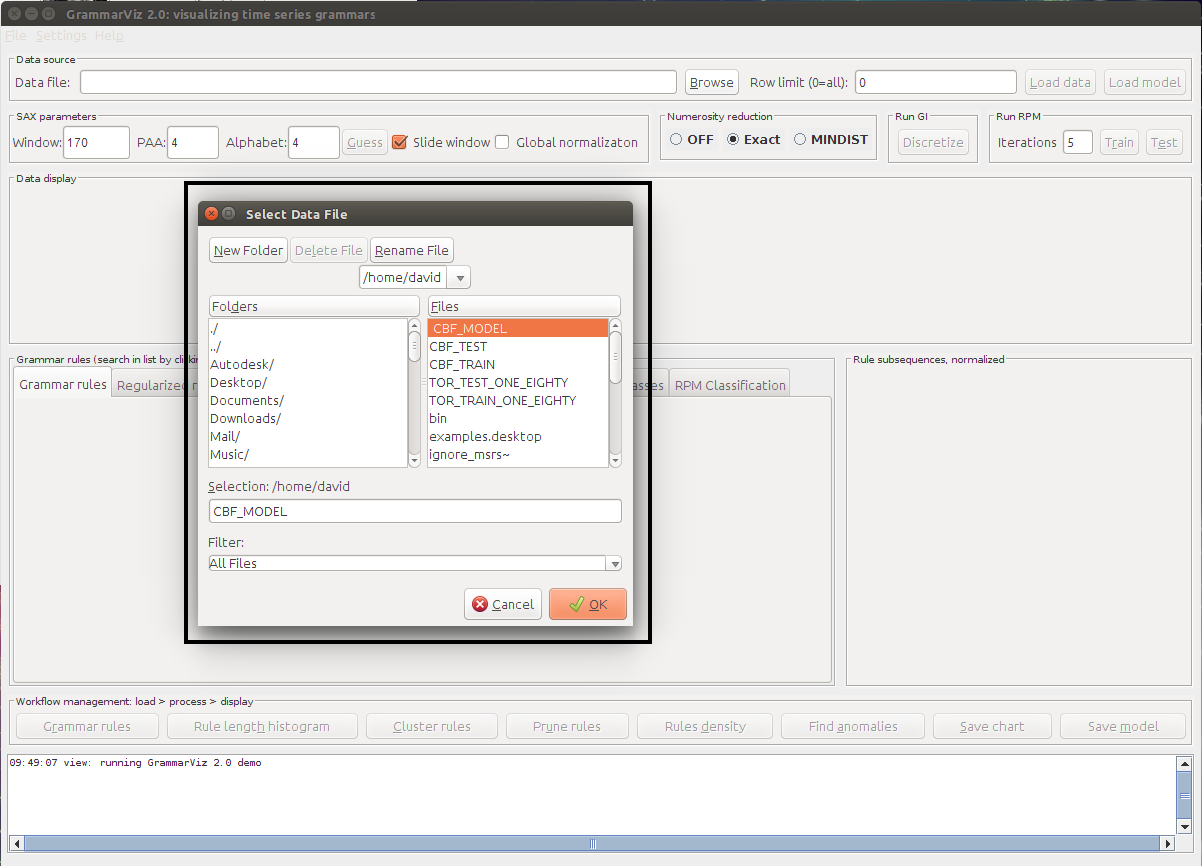
\includegraphics[width=\textwidth]{TSAT-load-model-step-2}
	\caption{Open the file browser prompt}
	\label{fig:TSAT-load-model-step-2}
\end{figure}

\newpage
\paragraph{Step 3}
Once the model has been selected, click the ``Load Model'' button and the model will be loaded into TSAT. If the data is not found during the loading step TSAT will ask for the location of the data using a file browser prompt, like in figure \ref{fig:TSAT-load-model-failed-data}, simple provide the data and the model will finish loading. 

\begin{figure}[H]
	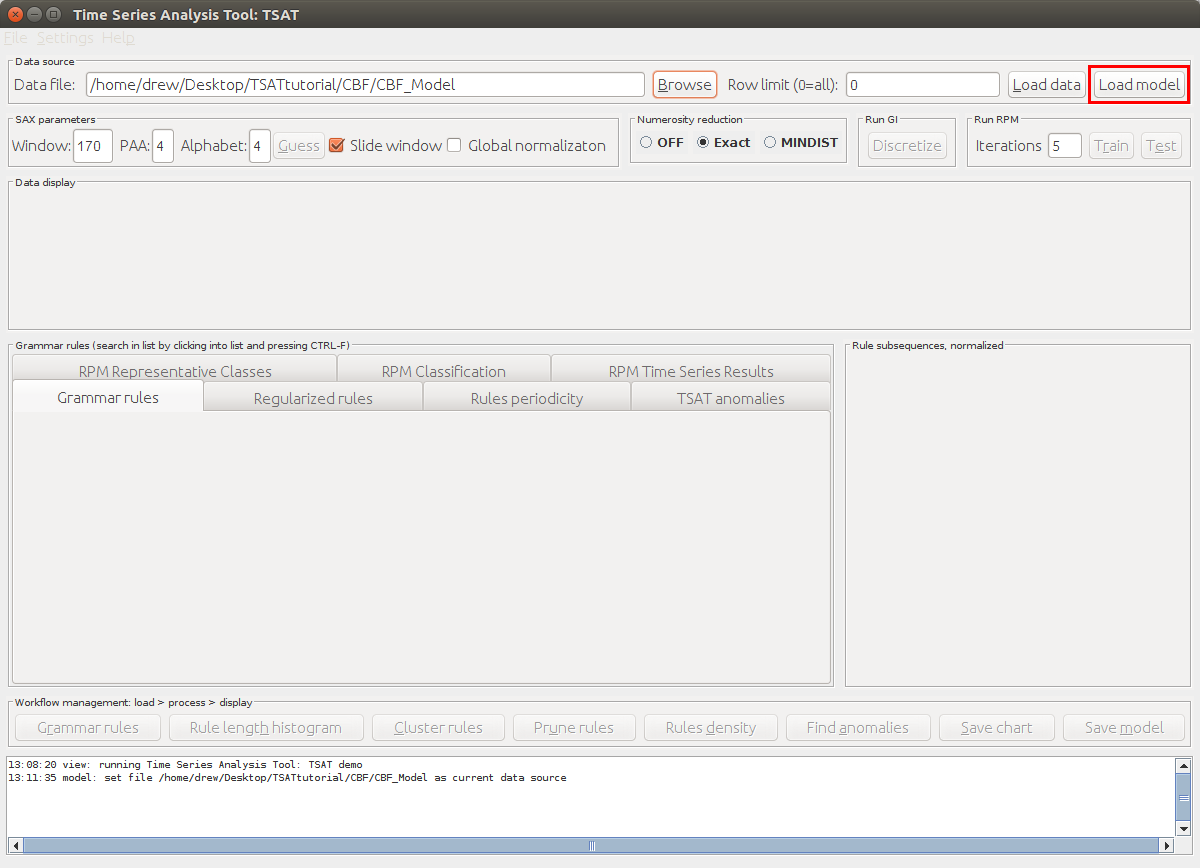
\includegraphics[width=\textwidth]{TSAT-load-model-step-3}
	\caption{Model loaded}
	\label{fig:TSAT-load-model-step-3}
\end{figure}

\begin{figure}[H]
	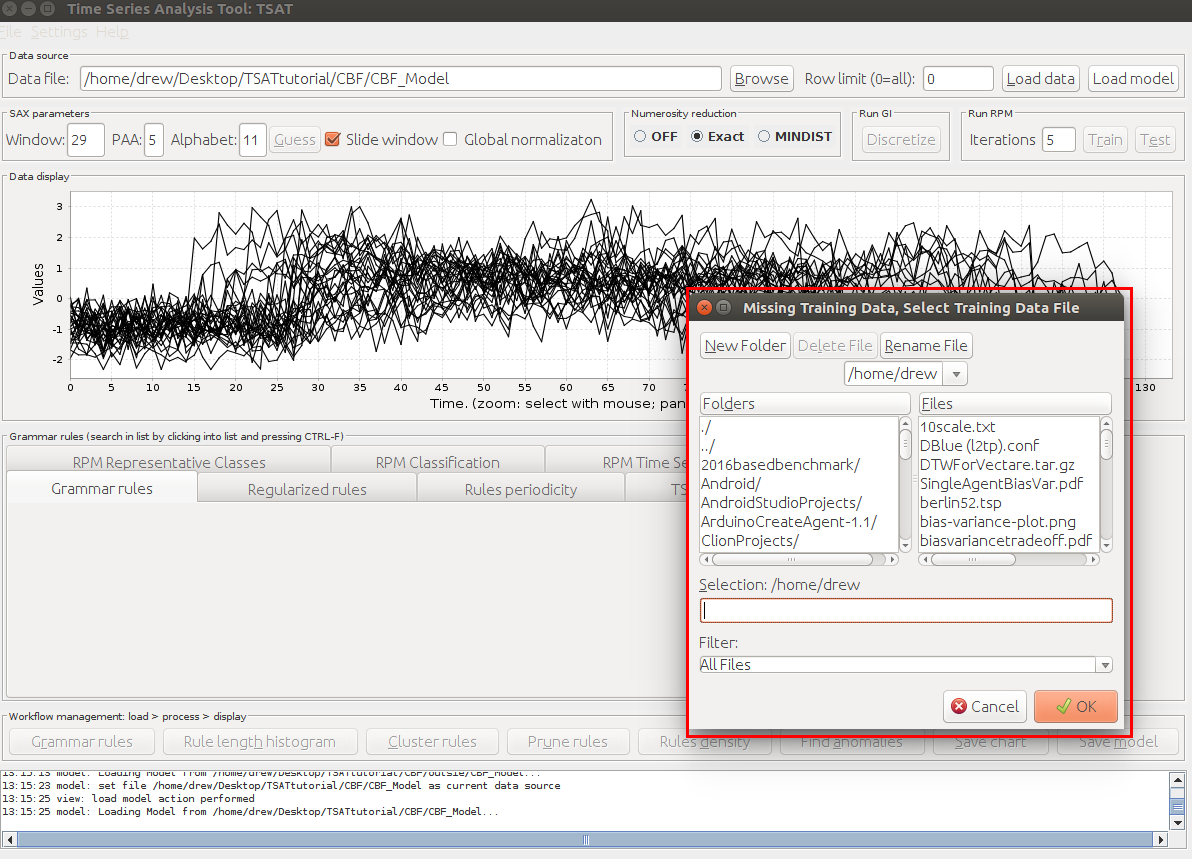
\includegraphics[width=\textwidth]{TSAT-load-model-failed-data}
	\caption{Missing training data file browser prompt}
	\label{fig:TSAT-load-model-failed-data}
\end{figure}

\subsection{Settings}
\label{RPMSettings}
There are a few options that can be changed when using RPM in TSAT, some of them have already been mentioned and will be covered again.

\subsubsection{Dynamic Time Warping}
Dynamic Time Warping, or DTW, is a method of measuring distance between two time series, this means how similar or different they are to each other. By default RPM uses Euclidean distance which is a simple and fast measurement, however it does not do well when the similar patterns between time series occur at different positions. This is where DTW comes in, it can handle temporal shifts in patterns and, depending on the data, can vastly improve the accuracy of the model. There is a cost however, DTW is a much slower operation and is very expensive to run so it is left as an option for the user. 

DTW also has another parameter called ``Window'' which can have dramatic effects on DTW both in how long it takes to run and its accuracy. The window size basically limits how far DTW will go to try to accurately try to match the two time series. A smaller window will stop DTW from trying to over match them and will take less time to compute. A larger window will take much longer to compute but can allow DTW to match patterns that are father apart. Choosing a good window size can be highly dependent on the data and what is being compared, and therefore some experimentation may be needed to find a good window size. There are a few good rules when choosing a window size, for one a window size greater then 10 will usually give bad results so 10 is considered a good starting point. Often for the more common types of data a 3-5 window size can be much better option with significant speed ups. Note DTW's window should not be confused with the Window size in the SAX parameters section of the main window, these are two different and distinct uses of the word window. 

\newpage
\paragraph{Step 1}
To change between Euclidean distance and DTW first open the settings menu:

``Settings''$\rightarrow$``TSAT options'' or press Ctrl+p. This will bring up the settings menu in figure \ref{fig:TSAT-settings-dialog}.

\begin{figure}[H]
	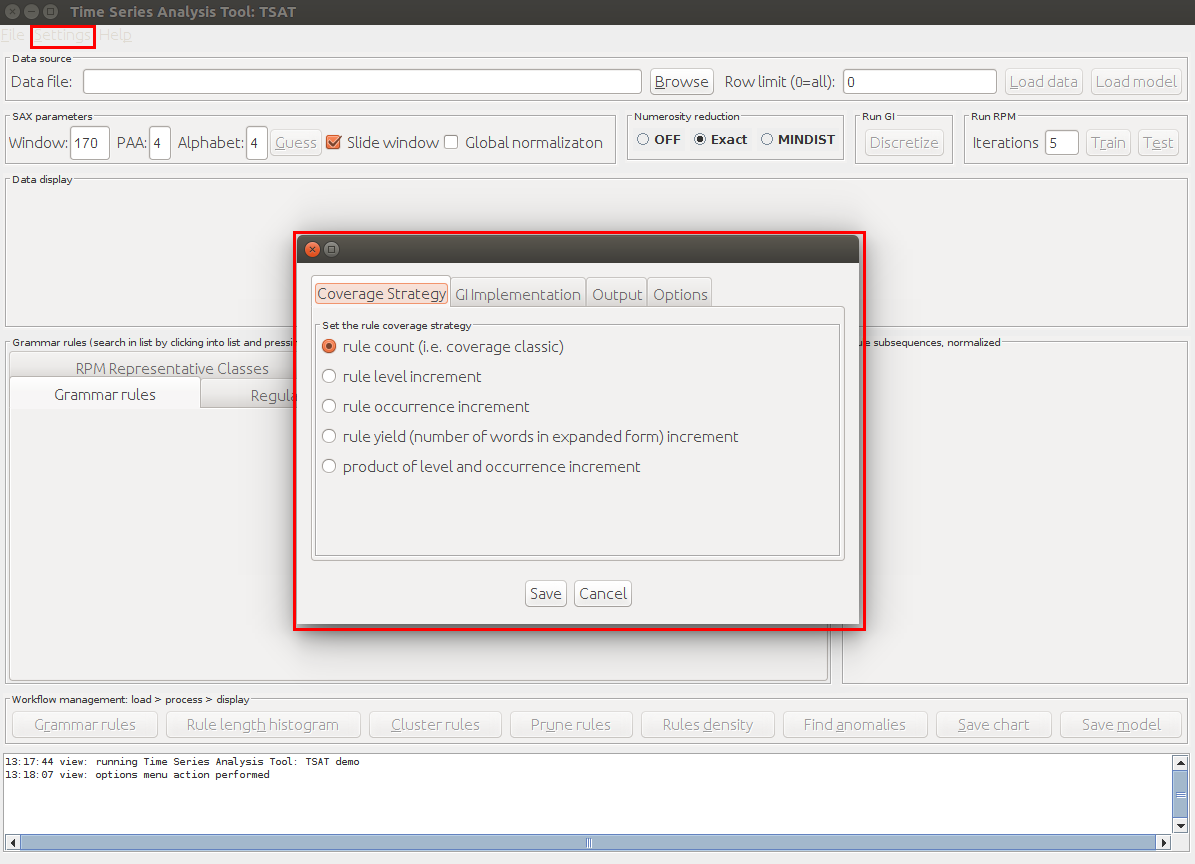
\includegraphics[width=\textwidth]{TSAT-settings-dialog}
	\caption{TSAT Settings Dialog}
	\label{fig:TSAT-settings-dialog}
\end{figure}

\newpage
\paragraph{Step 2}
Now click on the ``Options'' tab.

\begin{figure}[H]
	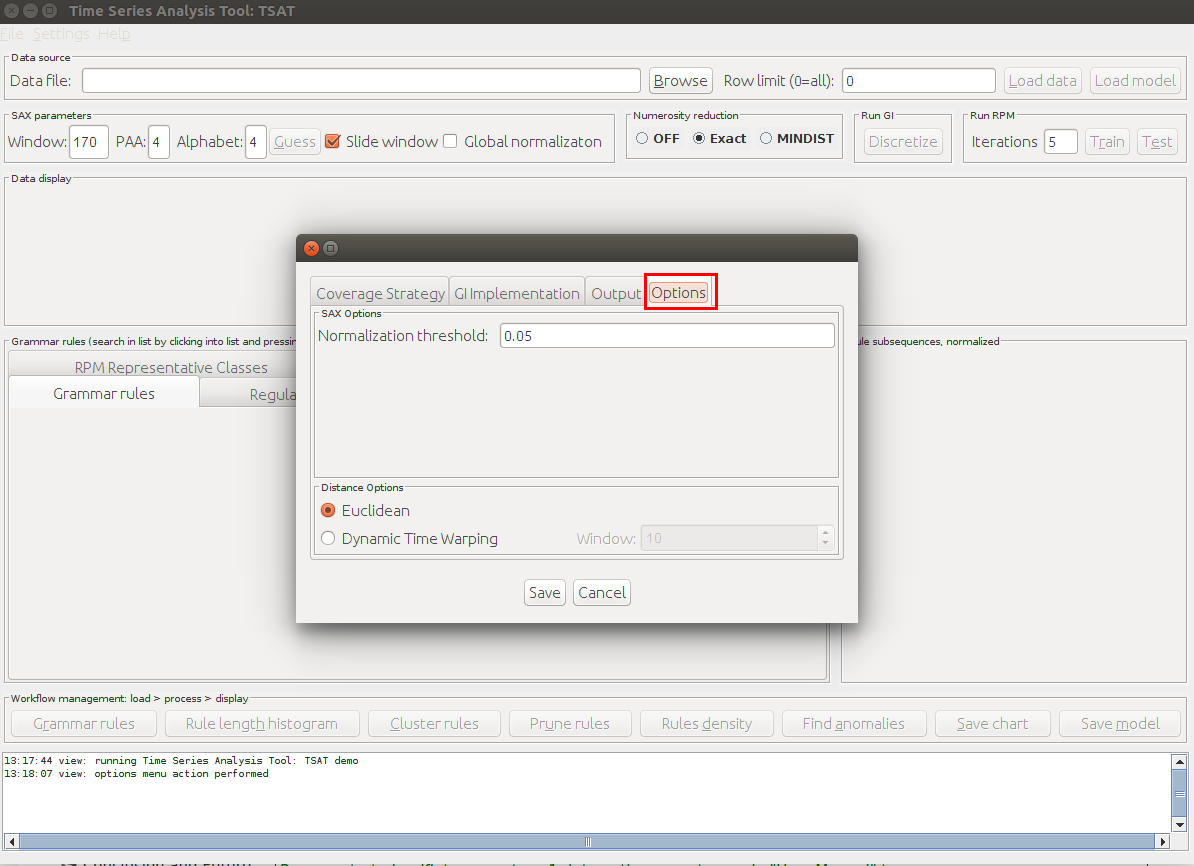
\includegraphics[width=\textwidth]{TSAT-settings-dialog-options}
	\caption{TSAT Settings Dialog Options}
	\label{fig:TSAT-settings-dialog-options}
\end{figure}

\newpage
\paragraph{Step 3}
Now select the ``Dynamic Time Warping'' option and the desired ``Window'' then click save.

\begin{figure}[H]
	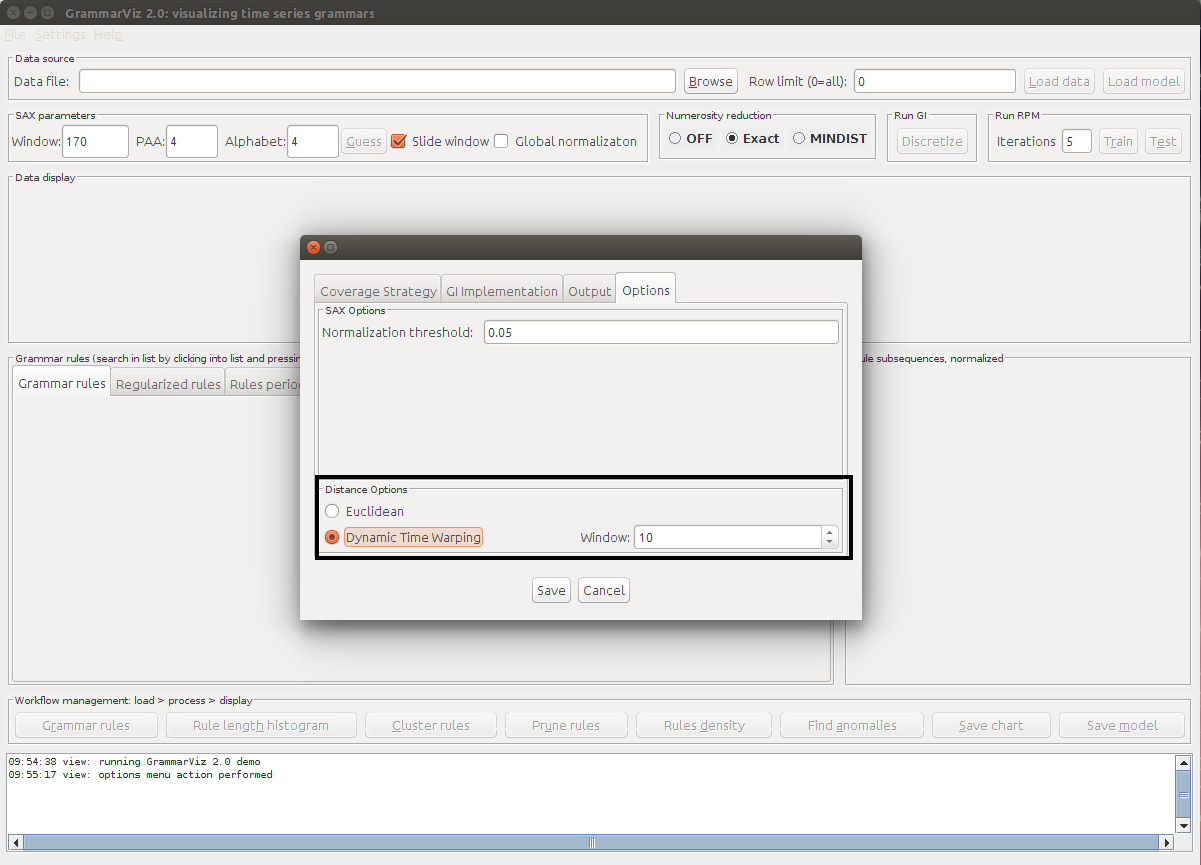
\includegraphics[width=\textwidth]{TSAT-settings-dialog-options-dtw}
	\caption{TSAT Settings Dialog Options DTW}
	\label{fig:TSAT-settings-dialog-options-dtw}
\end{figure}

\newpage
\subsubsection{Iterations}
During the operation of RPM it goes though a step that gets repeated many times. This step only stops under two conditions, a minimum threshold is met or if the maximum number of iterations are reached. The iterations setting found under the ``Run RPM'' section of the main window in TSAT is how the user can control the maximum number of iterations, figure \ref{fig:TSAT-iteration-setting}. The number of iterations can have an effect on how accurate the model can get, however the more iterations RPM runs through the longer it will take to complete. This becomes a balance between the quality of the model and the how long the training phase will take. It should also should be noted that RPM can stop before the maximum number of iterations is met if the model has reached an ideal state. However, this does not mean that all models will or even can reach an ideal state before the maximum number of iterations is reached, indeed some data sets may never return a model that meets the requirements. As RPM runs through the iterations the model should get better but the amount it gets better by can be come increasingly insignificant and therefore adding another 10 iterations may not add any significant results to the model. The only way to know if adding more iterations will improve the model is by experimentation which would involve training multiple times, increasing the maximum number of iterations every run until the testing results return no significant improvements.

\begin{figure}[H]
	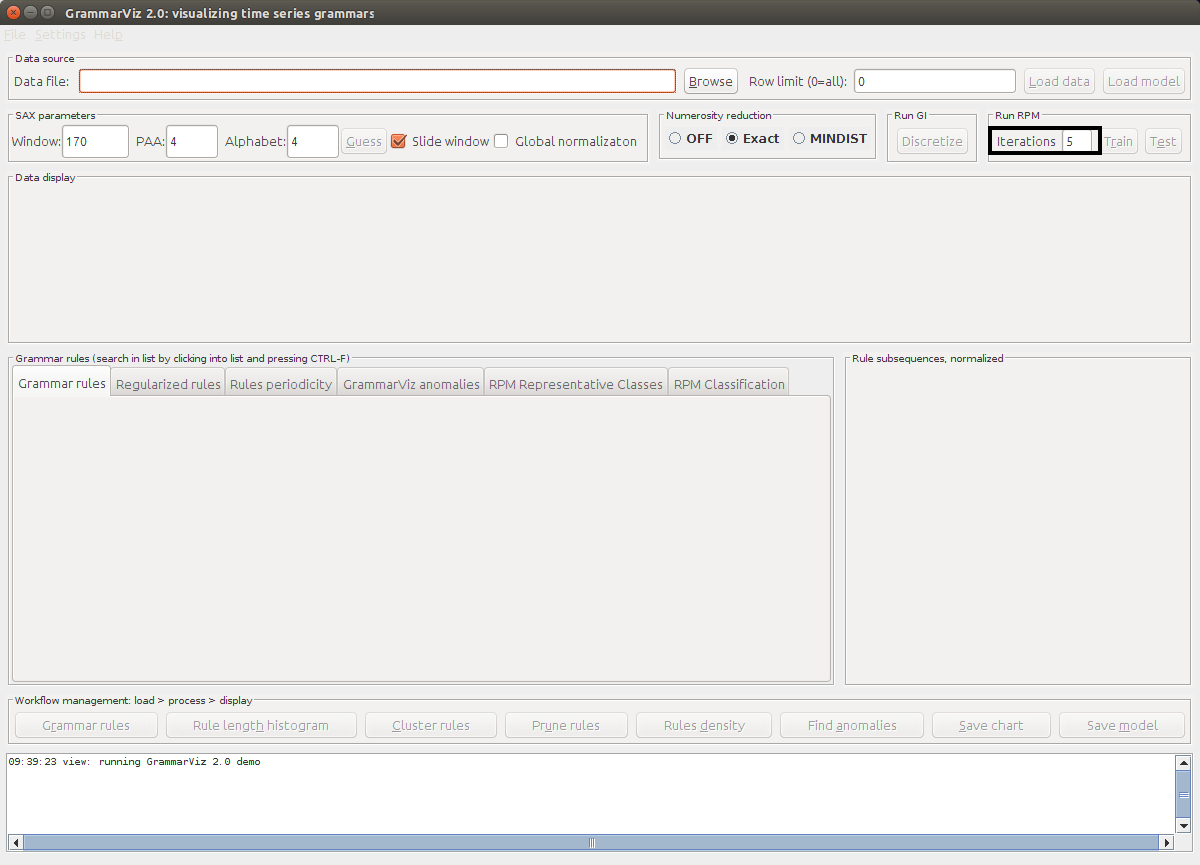
\includegraphics[width=\textwidth]{TSAT-iterations-setting}
	\caption{TSAT RPM Iteration Setting}
	\label{fig:TSAT-iteration-setting}
\end{figure}

\section{Motif Discovery}
\subsection{File format}
\subsection{Guide to Motif Discovery}


``Note however, that grammar induction step effectively mitigates improper sliding window selection.'' (\url{http://grammarviz2.github.io/grammarviz2_site/morea/motif/experience-m1.html}).

\section{Anomaly Detection}
\subsection{File format}
\subsection{Guide to Anomaly Detection}

\section{Error Messages}
\subsection{File Errors}
\subsection{RPM Errors}

\section{FAQs}

When training there must always be more than one example from each class label and there must be more than one label.

\paragraph{Installation}

This tutorial assumes that you are running Ubuntu 16.04 with Java 1.8 or greater installed.

\begin{allintypewriter}
	\noindent git clone https://github.com/dwicke/TSAT.git\\
	cd TSAT\\
	mvn package -Psingle\\
\end{allintypewriter}
This will create tsat-0.0.1-SNAPSHOT-jar-with-dependencies.jar in the target directory.  You can execute the jar and run the GUI by double clicking on it after changing its permissions:
\begin{verbatim}
chmod +x tsat-0.0.1-SNAPSHOT-jar-with-dependencies.jar
\end{verbatim}  


To run the GUI from a shell you can do:
\begin{verbatim}
$ java -Xmx2g -jar target/tsat-0.0.1-SNAPSHOT-jar-with-dependencies.jar 
\end{verbatim}

The -Xmx2g allocates max of 2Gb of memory for the software.



\bibliographystyle{ieeetr}
\bibliography{citations}

\end{document}
